% basic settings
\documentclass[a4paper,12pt]{article}
\usepackage[utf8]{inputenc}
\usepackage[czech]{babel}

% customizations
\usepackage{parskip} % paragraph indentation will be suppressed, instead there will be a space after
\usepackage[ddmmyyyy]{datetime} \renewcommand{\dateseparator}{.} % enables \today as dd.mm.yyyy
\usepackage{amsmath}
\usepackage{xcolor}
\usepackage{hyperref}
\usepackage{float}
\usepackage{graphicx}
\usepackage[left = 2.0cm, right = 2.0cm, top = 2.5cm, bottom = 2.5cm]{geometry}

\begin{document}

\def\D{\mathrm{d}} % non-italic differential sign

\begin{center}
\LARGE\textbf{Protokol z projektu} \\
\vspace{2cm}
\large{
	Projekt na Numerické metody pro inženýry (P413003) \\
	Zadání č. 9 \\
	Vypracoval Ing. Jiří Zbytovský (\textcolor{blue}{\underline{\href{mailto:zbytovsi@vscht.cz}{email}}}) \\
	Odevzdáno \today
}
\end{center}



\newpage
\section*{Úloha 1}
Původní diferenciální rovnice popisující izotermní vnitřní difúzi v porézením katalyzátoru:
\begin{equation}
	\frac{\D^2 y}{\D x^2} + \frac{a}{x} \frac{\D y}{\D x} = \Phi^2 y^n
\end{equation}

S okrajovými podmínkami:
\begin{align}
	\frac{\D y}{\D x} (0) &= 0
	\\
	y(1) &= 1
\end{align}
Kde $y$~je bezrozměrná koncentrace, $x$~bezrozměrná souřadnice poloměru (0~je střed částice, 1~je její okraj), $a=1$~charakterizuje tvar částice (váleček), $\Phi=1$~Thieleho modul a $n=2$~řád reakce.

Diferenciální rovnici (DR) druhého řádu je třeba nahradit soustavou dvou DR prvního řádu, kde závislé proměnné jsou $y_1$ a $y_2$:
\begin{align}
	y_1 &= y
	\\
	y_2 &= y' = \D y / \D x
\end{align}

Výsledkem je tato soustava DR (s dosazením $\Phi$, $n$, $a$):
\begin{align}
	\frac{\D y_1}{\D x} = y_1' = f_1(x,y_1,y_2) &= y_2
	\\
	\frac{\D y_2}{\D x} = y_2' = f_2(x,y_1,y_2) &= -\frac{a}{x} y_2 + \Phi^2 y_1^n = y_1^2 - y_2 / x
\end{align}

S okrajovými podmínkami:
\begin{align}
	y_2(0) &= 0
	\\
	y_1(1) &= 1
\end{align}

Tento okrajový problém nyní řeším převedením na počáteční problém metodou střelby s variačními rovnicemi.
Volím proto $\eta$ jako odhad počáteční hodnoty $y_1(0) = \eta$ (zatímco $y_2(0)$ je dáno přesně).
Volba $\eta$ je přijatelná tehdy, když je přibližně splněna okrajová podmínka vyjádřená jako $\phi(\eta) = 0$, kde funkce $\phi$ vyjadřuje residuum rovnice okrajové podmínky při odhadu $\eta$:
\begin{equation}
	\phi(\eta) = y_1(1, \eta) - 1
\end{equation}

Aby byla přibližně splněna okrajová podmínka, použiji Newtonovu metodu na získání vhodnější hodnoty $\eta$ (iteruji s čítačem $k$):
\begin{equation}
	\eta_{k+1} = \eta_{k} + \frac{\phi(\eta_k)}{\phi'(\eta_k)}
\end{equation}

Kde $\phi'(\eta_k)$ je derivace $\phi$ podle $\eta$. Pro její vyčíslení zavedu variační rovnice pro nové závislé veličiny $p_1$, $p_2$:
\begin{align}
	p_1 &= \frac{\partial y_1}{\partial \eta}
	\\
	p_2 &= \frac{\partial y_2}{\partial \eta}
\end{align}

Jejich derivace lze vyjádřit řetízkovým pravidlem, čímž jsou získány další diferenciální rovnice do výše uvedené soustavy DR:
\begin{align}
	p_1' &=
	\frac{\partial p_1}{\partial x} =
	\frac{\partial^2 y_1}{\partial x \partial \eta} =
	\frac{\partial f_1}{\partial \eta} =
	\frac{\partial f_1 \partial y_1}{\partial y_1 \partial \eta} + \frac{\partial f_1 \partial y_2}{\partial y_2 \partial \eta} =
	\frac{\partial f_1}{\partial y_1} p_1 + \frac{\partial f_1}{\partial y_2} p_2 =
	p_2
	\\
	p_2' &=
	\frac{\partial p_2}{\partial x} =
	\frac{\partial^2 y_2}{\partial x \partial \eta} =
	\frac{\partial f_2}{\partial \eta} =
	\frac{\partial f_2 \partial y_1}{\partial y_1 \partial \eta} + \frac{\partial f_2 \partial y_2}{\partial y_2 \partial \eta} =
	\frac{\partial f_2}{\partial y_1} p_1 + \frac{\partial f_2}{\partial y_2} p_2 =
	2 y_1 p_1 - p_2 / x
\end{align}

S odpovídajícími počátečními podmínkami:
\begin{align}
	p_1(0) &= \frac{\partial y_1}{\partial \eta}(0) = 1
	\\
	p_2(0) &= \frac{\partial y_2}{\partial \eta}(0) = 0
\end{align}

Nyní lze vyjádřit derivaci $\phi'(\eta_k)$:
\begin{equation}
	\phi' = \frac{\partial \phi}{\partial \eta} = \frac{\partial (y_1(1, \eta) - 1)}{\partial \eta} = p_1(1, \eta)
\end{equation}

A tedy dosadit do vzorce pro Newtonovu metodu:
\begin{equation}
	\eta_{k+1} = \eta_{k} + \frac{y_1(1, \eta) - 1}{p_1(1, \eta)}
\end{equation}

Řeším tedy následující počáteční problém pomocí Runge-Kuttovy metody (použita implementace z open-source knihovny \textcolor{blue}{\underline{\href{https://scipy.org/}{scipy}}}).
\begin{align}
\label{ode1}
	y_1' &= y_2 &&
	y_1(0) = \eta_k
	\\
\label{ode2}
	y_2' &= y_1^2 - y_2 / x &&
	y_2(0) = 0
	\\
	p_1' &= p_2 &&
	p_1(0) = 1
	\\
	p_2' &= 2 y_1 p_1 - p_2 / x &&
	p_2(0) = 0
\end{align}

Postup zahájím volbou např. $\eta = \tfrac{1}{2}$ a výše uvedený postup iteruji přes $k$. \\
Iteraci $k$ ukončím tehdy, když $|\eta_{k+1} - \eta_{k}| < \epsilon$, kde $\epsilon$ je zvolená mez pro stanovení konvergence.
Následně řeším soustavu DR bez variačních rovnic, čili pouze rovnice~\ref{ode1}~a~\ref{ode2}. \\
Řešením soustavy jsou vektory $x$, $y_1$ a $y_2$, což je výsledek této úlohy.

Implementace tohoto postupu je v souboru \textit{app/uloha\_1.py}. \\
Výsledky jsou uvedeny v poslední kapitole.



\newpage
\section*{Úloha 2}
Původní parciální diferenciální rovnice (PDR) popisující dynamiku vnitřní difúze v částici katalyzátoru s reakcí druhého řádu:

\begin{equation}
	\frac{\partial u}{\partial t} = \frac{\partial^2 u}{\partial x^2} - \delta u^2
\end{equation}

S počáteční podmínkou:
\begin{align}
	u(x,0) = 4 (x - \tfrac{1}{2})^2 && x \in \langle0, 1\rangle
\end{align}

A s okrajovými podmínkami:
\begin{align}
	u(0,t) = u(1,t) = 1 && t > 0
\end{align}

Přičemž $u$ značí koncentraci, $x$~prostorovu souřadnici průměru (od kraje ke kraji), $t$~čas a $\delta$~rychlostní konstantu reakce (všechny veličiny v bezrozměrném tvaru).\\
Pozn.: před člen s druhou derivací dle $x$~by bylo možné přidat $D$, bezrozměrný difúzní koecifient, aby byl systém plně parametrizován.

Tato PDR bude řešena metodou Crankovou-Nicholsonové pro $t \in \langle0, 1\rangle$~a $\delta = 1$.
Aby ji bylo možné touto metodou řešit, je třeba provést linearizaci.

Nejprve však na intervalech $x \in \langle0, 1\rangle$, $t \in \langle0, 1\rangle$ tabeluji hodnoty nezávislých veličin:
\begin{align}
	x_i = i h && h &= 1/n && i = 0...n
	\\
	t_j = j k && k &= 1/m && j = 0...m
\end{align}

Řešení tedy budu hledat na této množině:
\begin{equation}
	D^{h,k} = \left\{ (x_i, t_j), i = 0...n, j = 0...m \right\}
\end{equation}

Na této množině provedu náhradu derivací diferenčními formulemi, abych získal přibližné řešení: $u(x_i, t_j) \approx u_i^j$ \\
Takto vyjádřím derivace v bodě $i$, $j+1$:
\begin{align}
	\frac{\partial u}{\partial t}(x_i, t_{j+1}) &=
	\frac{u_i^{j+1} - u_i^j}{k}
	\\
	\frac{\partial^2 u}{\partial x^2}(x_i, t_{j+1}) &=
	\frac{1}{2} \frac{u_{i-1}^{j+1} - 2 u_i^{j+1} + u_{i+1}^{j+1}}{h^2} +
	\frac{1}{2} \frac{u_{i-1}^j - 2 u_i^j + u_{i+1}^j}{h^2}
\end{align}

Dále, nelineární člen $(u_{i}^{j+1})^2$ linearizuji jako $u_{i}^{j} u_{i}^{j+1}$

Aproximaci PDR na množině $D^{h,k}$ pak lze sestavit takto:

\begin{equation}
	\frac{u_i^{j+1} - u_i^j}{k} =
	\frac{1}{2} \frac{u_{i-1}^{j+1} - 2 u_i^{j+1} + u_{i+1}^{j+1}}{h^2} +
	\frac{1}{2} \frac{u_{i-1}^j - 2 u_i^j + u_{i+1}^j}{h^2} +
	u_{i}^{j} u_{i}^{j+1}
\end{equation}

Pro přehlednost definuji $\alpha = k / h^2$ a PDR upravím:
\begin{equation}
\label{apxPDR}
	-\tfrac{\alpha}{2} u_{i-1}^{j+1} +
	(1 + \alpha + k u_i^j) u_i^{j+1} -
	\tfrac{\alpha}{2} u_{i+1}^{j+1} =
	\tfrac{\alpha}{2} \left( u_{i-1}^j - 2 u_i^j + u_{i+1}^j \right) + u_i^j
\end{equation}

Řešením této aproximované PDR je matice $U = \left( u_i^j \right)$.
Postup k jejímu získání je následující: na počátku znám první řádek $u_i^0 = 4(x_i - \tfrac{1}{2})^2$ a postupně získávám další řádky (iteruji $j+1$).

Z řádku $j+1$ vždy znám hodnoty $u_0^{j+1} = u_n^{j+1} = 1$.

Zbývající hodnoty $u_i^{j+1}$ v $i=1...(n-1)$ získám řešením soustavy $(n-1)$ lineárních rovnic~\ref{apxPDR}, kde každá tato rovnice vyjadřuje platnost PDR pro bod $u_i^{j+1}$ v daném $i$.

Tato soustava je zapsána maticově:
\begin{equation}
	A^j u^{j+1} = b^j
\end{equation}

Maticový zápis PDR~\ref{apxPDR} je rozepsán pro příklad s $n=5$:
\begin{equation}
\begin{pmatrix}
	\beta & \tfrac{\alpha}{2} & 0 & 0 \\
	\tfrac{\alpha}{2} & \beta & \tfrac{\alpha}{2} & 0 \\
	0 & \tfrac{\alpha}{2} & \beta & \tfrac{\alpha}{2} \\
	0 & 0 & \tfrac{\alpha}{2} & \beta
\end{pmatrix}
\cdot
\begin{pmatrix}
	u_1^{j+1} \\ u_2^{j+1} \\ u_3^{j+1} \\ u_4^{j+1}
\end{pmatrix}
=
\begin{pmatrix}
	\tfrac{\alpha}{2} \left( 1 - 2 u_1^j + u_2^j \right) + u_1^j + \tfrac{\alpha}{2} \\
	\tfrac{\alpha}{2} \left( u_{i-1}^j - 2 u_i^j + u_{i+1}^j \right) + u_i^j \\
	\tfrac{\alpha}{2} \left( u_{i-1}^j - 2 u_i^j + u_{i+1}^j \right) + u_i^j \\
	\tfrac{\alpha}{2} \left( u_{n-2}^j - 2 u_{n-1}^j + 1 \right) + u_{n-1}^j + \tfrac{\alpha}{2} \\
\end{pmatrix}
\end{equation}
Kde člen $\beta$ je definován jako $1 + \alpha + k u_i^j$

Řešení soustavy rovnic je realizováno pomocí algoritmu z open-source knihovny \textcolor{blue}{\underline{\href{https://numpy.org/}{numpy}}}.\\
Tímto postupem je řádek po řádku získána celá matice $U$.

Implementace tohoto postupu je v souboru \textit{app/uloha\_2.py}. \\
Výsledky jsou uvedeny v poslední kapitole.



\newpage
\section*{Výsledky}
Průběh řešení DR z úlohy 1 je znázorněn na grafu níže.
Řešení je na pohled hladké, bez oscilací, a splňuje okrajové podmínky se zadanou přesností.
\begin{figure}[H]
\begin{center}
	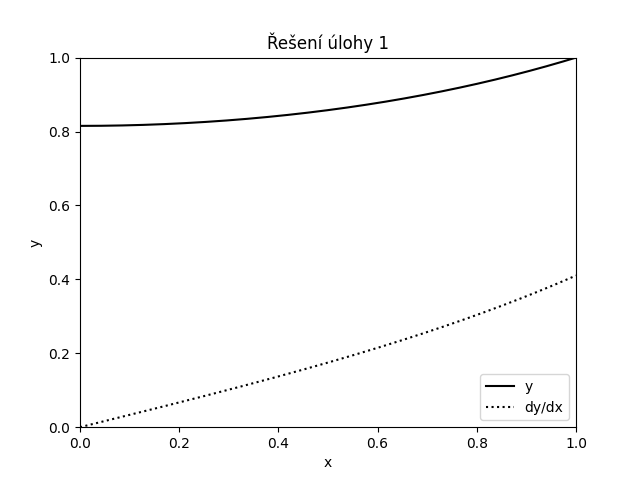
\includegraphics[width=0.75\textwidth]{uloha_1.png}
\end{center}
\end{figure}

Průběh řešení PDR z úlohy 2 je znázorněn na grafu níže.
Není pozorována oscilace, průběh funkce je v obou směrech hladký.
\begin{figure}[H]
\begin{center}
	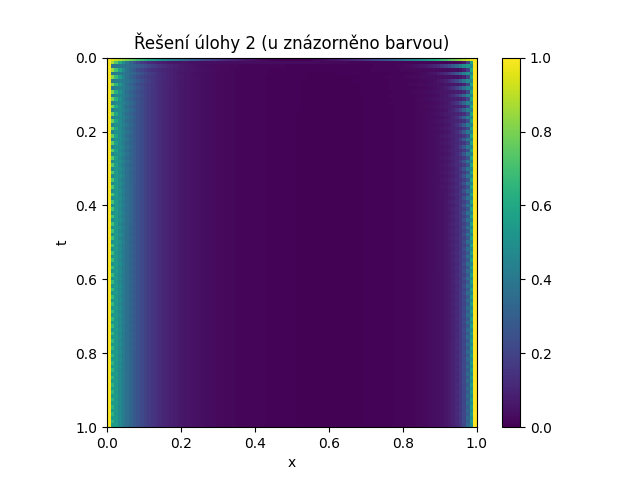
\includegraphics[width=0.75\textwidth]{uloha_2.png}
\end{center}
\end{figure}

\end{document}
